\documentclass[12pt]{article}
\usepackage{url,amsmath,graphicx,tabularx,array}
\usepackage[hscale=0.7,vscale=0.8]{geometry}
\setlength{\parskip}{1ex} %--skip lines between paragraphs
\setlength{\parindent}{0pt} %--don't indent paragraphs

%-- Commands for header
\renewcommand{\title}[1]{\textbf{#1}\\}
\renewcommand{\line}{\begin{tabularx}{\textwidth}{X>{\raggedleft}X}\hline\\\end{tabularx}\\[-0.5cm]}
\newcommand{\leftright}[2]{\begin{tabularx}{\textwidth}{X>{\raggedleft}X}#1%
& #2\\\end{tabularx}\\[-0.5cm]}

%\linespread{2} %-- Uncomment for Double Space
\begin{document}
%%%%%%%%%%%%%%%%%%%%%%%%%%%%%%%%%%%%%%%%%%%%%%%%%%%%%%%%%%%%%%%%%%%%%%%%%%%%%%%%%

\title{ECE 446 – FALL 2014 COMPUTER PROJECT 1}
\line
\leftright{\today}{Md. Iftekhar Tanveer} %-- left and right positions in the header

\section{Estimating Spectrum of White Noise}
The noise array was generated by the following command:
\begin{verbatim}
Noise = .05*(rand(512000,1)-.5);
\end{verbatim}
``rand'' generates uniformly distributed random numbers from 0 to 1. So, mean of $\text{rand}(512000,1)-0.5$ is zero. Variance of this random number is $2.0833\times10^{-4}$ as calculated below:
\begin{equation}
\begin{split}
 & \int_{0}^{1}\{0.05(u-0.5)\}^{2}du\\
= & \int_{0}^{1}0.0025(u^{2}-0.1u+0.25)du\\
= & \left[0.0025\frac{u^{3}}{3}-0.0025\frac{u^{2}}{2}+6.25\times10^{-4}\right]_{0}^{1}\\
= & 2.0833\times10^{-4}
\end{split}
\end{equation}
The spectral estimate of the noise is shown in Fig. \ref{fig:spectralEst}.
\begin{figure}[h]
    \centering
    \includegraphics[width=0.75\textwidth]{spectralestimate}
    \caption{Plot of the Noise Spectrum (NoiseSpectrum2048)}
    \label{fig:spectralEst}
\end{figure}
We see that the spectral estimate is uniformly distributed over the whole frequency range. The mean value of the spectral estimate is $2.0790\times10^{-4}$. which is very close to our calculated value ($2.0833\times10^{-4}$).

\textbf{Effect of FFTsize}
Frequency spectrum for different values of FFTsize is shown in Fig. \ref{fig:spectralEst_FFTsize}.
\begin{figure}[h]
    \centering
    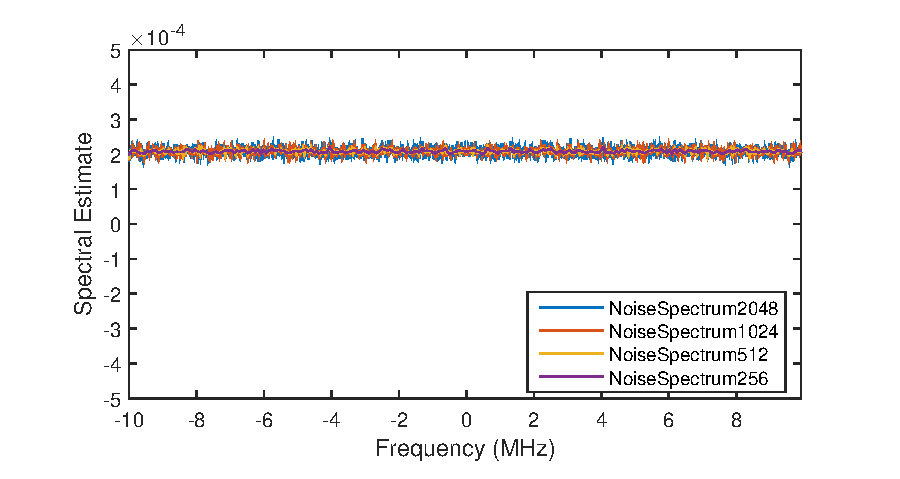
\includegraphics[width=0.8\textwidth]{spectralestimate_FFTsize}
    \caption{Plot of the spectral estimates of the white noise with four different FFTsizes. }
    \label{fig:spectralEst_FFTsize}
\end{figure}
\begin{figure}[h]
    \centering
    \includegraphics[width=0.8\textwidth]{spectralestimate_FFTsize_Zoomed}
    \caption{A zoomed version of the spectral estimates}
    \label{fig:spectralEst_FFTsize_Zoomed}
\end{figure}
A zoomed version of Fig. \ref{fig:spectralEst_FFTsize}. is shown in Fig. \ref{fig:spectralEst_FFTsize_Zoomed}. It is evident from the plots that the estimates with larger FFTsize is actually giving higher variance in the signal. To confirm this, I used the ``var'' command in MATLAB to calculate the variances of each estimate and found the following values.
\begin{verbatim}
K>> var(NoiseSpectrum2048)

ans =

   1.3260e-10

K>> var(NoiseSpectrum1024)

ans =

   6.3638e-11

K>> var(NoiseSpectrum512)

ans =

   2.9683e-11

K>> var(NoiseSpectrum256)

ans =

   1.5274e-11
\end{verbatim}
The results of the var commands shown above confirms the fact that the larger the FFTsizes, the larger the variances of the spectral estimates. This is due to the fact that, with larger FFTsize, we needed to increase the step-size (skip) as well. As a result, there were fewer number of sections over which we could take an average of the power spectral density. This resulted in a poorer approximation of the spectral density with larger FFTsizes. 

\section{LTI System with White Noise Input}
In this section, the output of the following LTI system is calculated while the input is the same white noise discussed in previous section.
\begin{verbatim}
y[n] = x[n] - 0.9x[n]
\end{verbatim}
Fig. \ref{fig:spectralEst_transform} presents the spectral estimates of the output signal. It shows the estimates for four different FFTsizes.
\begin{figure}[h]
    \centering
    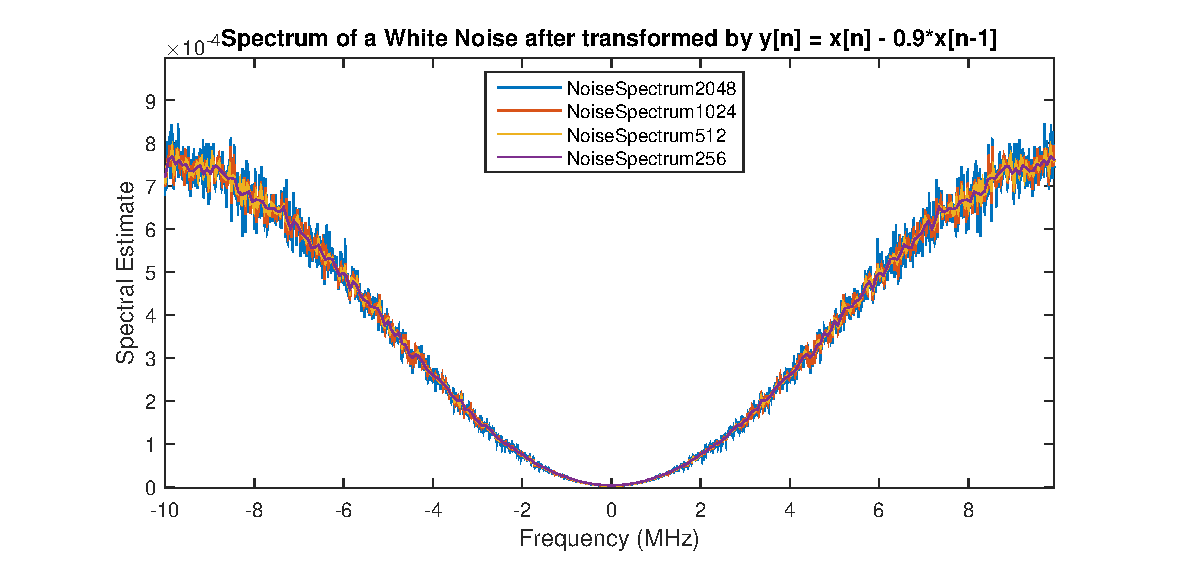
\includegraphics[width=1\textwidth]{spectralestimate_transform}
    \caption{White noise after being transformed by an LTI system}
    \label{fig:spectralEst_transform}
\end{figure}

To check if it a correct representation, I calculated the Spectral Density of the system. Input-output relation of the LTI system is as follows:
\[
y[n]=x[n]-0.9x[n-1]
\]
So, the impulse response will be as follows (by replacing the input
to an impulse):

\[
h[n]=\delta[n]-0.9\delta[n-1]
\]


Therefore, the frequency response of the transfer function is:
\begin{align*}
\text{H}(e^{jw}) & =1-0.9e^{-jw}\\
 & =1-0.9cos(w)+j0.9sin(w)\\
\implies\left|\text{H}(e^{jw})\right|^{2} & =(1-0.9cos(w))^{2}+(0.9sin(w))^{2}\\
 & =1-1.8cos(w)+0.81cos^{2}(w)+0.81sin^{2}(w)\\
 & =1-1.8cos(w)+0.81\\
 & =1.81-1.8cos(w)
\end{align*}

The output that we see follows the shape of this equation. However, in the actual spectrum of the output, this function will be scaled by the square of variance of the input white noise. As we notice from Fig \ref{fig:spectralEst_transform}, the error in the estimation is more prominent in the higher frequency components.

\section{Calculating Spectograph of Ashokan Farewell.wav}
\begin{figure}
    \centering
    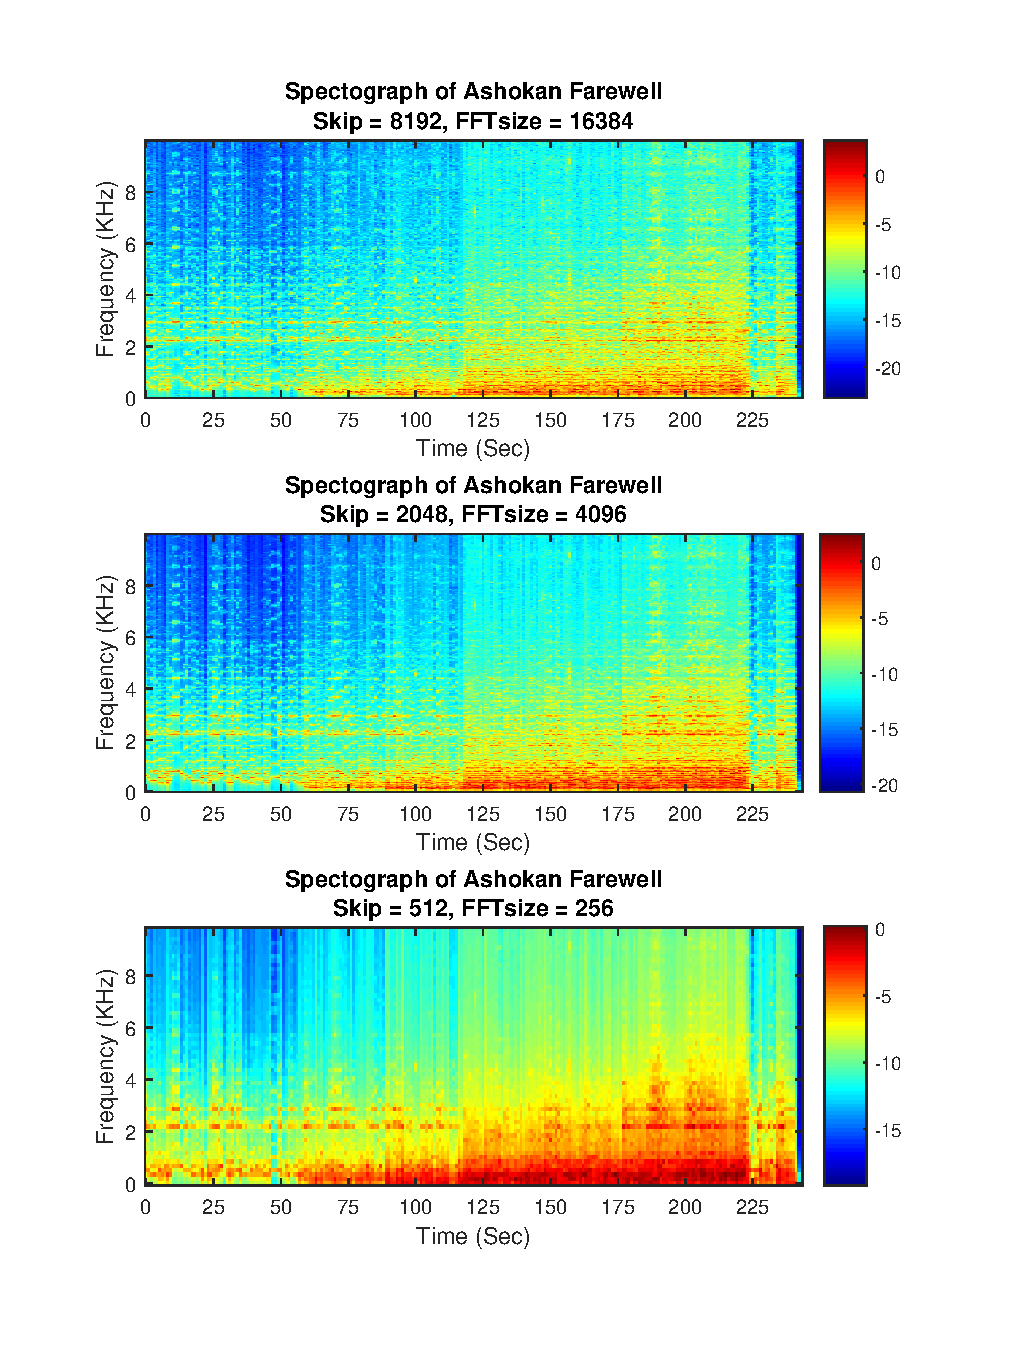
\includegraphics[width=1.07\textwidth]{spectra}
    \caption{Spectographs of the sound file ``Ashokan Farewell.wav''. The spectographs were drawn three times with three different sets of parameter Skip and FFTsize}
    \label{fig:spectra}
\end{figure}
The spectograph of the Ashokan Farewell sound file is shown in Fig. \ref{fig:spectra}. The spectographs were drawn for three different sets of parameters as indicated in the corresponding title. The topmost spectograph uses a FFTsize of 16384 samples. On the other hand, the second spectograph uses only 4096 samples in the Discrete Fourier Transform (DFT). Although this introduces a drop of resolution along y axis, it is not particularly noticeable. However, it uses a lower skip size. This makes the second spectograph a better estimation than the first one -- because -- the smaller step size results in a larger number of sections. As a result, the average will produce better estimate.

However, the third spectograph is worse in comparison to both first and the second spectograph. It uses a FFTsize of 256 and skip size of 512. Only 256 samples along the y axis does not provide enough resolution. As a result, the spectograph appeared to be smeared over the frequency axis. Moreover, since the Skip size is larger than the FFTsize, the spectograph is not actually using all the information available in the signal. It is discarding half of the signal before calculating the FFT. As a result, the spectograph will not represent accurate information.

\section{Analysis of Relationship between Spectra and the Music}
I noticed two important points while analyzing the Spectra and the Music. The first point is related to musical instrument and the spectral representation. During the first 60 (appx.) seconds only violin was being played. This corresponded to a distinct pattern in the frequency spectra. Only a discrete components of frequency (e.g. 1.45kHz, 2.14kHz, 2.88khz etc.) was showing higher energy depending on the notes being played. After about 60 seconds, when the guitar was being played along with the violin, there was a change in the spectograph. This time, the lower ranges in the frequency spectrum (0 - 1.5kz) also started to show high energy components. From this observation, I came to a conclusion that violin plays at higher frequency range than guitar. At around 150 seconds, when the piano was being played, the patterns in the frequency components were changed. The distinct patterns of violin on the frequency range ( between 1.5kHz to 4 kHz) showed much lower energy during this time period. This pattern reappeared in around 200 sec, where the lead violin was being played again. 

Another point that I noticed is -- the more the number of instruments were being played, the more area in the spectograph was turning red. This means, when there was higher energy in time domain, the frequency domain also showed higher energy. This effect can be explained by Parsival's theorem which mentions that the energy is same over time and frequency domain representation of the signal.

\section{CODE}
    \begin{verbatim}
%------------------------------------------------------------------
%  ECE 446 Computer Project 1 Fall 2014
%  Project Done by: M. Iftekhar Tanveer (itanveer@cs.rochester.edu)
%  This project was coded and tested in MATLAB R2014b
%  Please run the scripts in MATLAB 2014b for correct execution
%------------------------------------------------------------------
%
% Part 1: Plot spectrums of noises
%
function projMain
clc;clear;
Fs = 20; % Given in question. Mhz is assumed

% Generate the noise signal
Noise = .05*(rand(512000,1)-.5);

% Estimate Spectrum
NoiseSpectrum2048 = EstimateSpectrum(Noise,1024,2048);

% Plot 64 Samples from the Spectrum
figure(1);
N_x = 64;
sftSpec = fftshift(NoiseSpectrum2048);
N = length(sftSpec); % Number of samples
N_2 = floor(N/2); % Center index
sftSpec = sftSpec(N_2-N_x:N_2+N_x-1); %Shift
% Plotting on log scale for better representation
plot(sftSpec);
ylabel('Spectral Estimate');
xlabel('Samples');
axis ([0,length(sftSpec),-0.0005,0.0005]);

% Additional spectrums of noise.
NoiseSpectrum1024 = EstimateSpectrum(Noise,512,1024);
NoiseSpectrum512 = EstimateSpectrum(Noise,256,512);
NoiseSpectrum256 = EstimateSpectrum(Noise,128,256);

% Plot all the Spectrums
figure(2);
plotSpectrums({NoiseSpectrum2048,NoiseSpectrum1024,NoiseSpectrum512, ...
    NoiseSpectrum256},Fs,{'NoiseSpectrum2048','NoiseSpectrum1024', ...
    'NoiseSpectrum512','NoiseSpectrum256'});

% -------------------------------------------------------------------
% Part 2: Noise passed through a LTI system: y[n] = x[n] - 0.9*x[n-1]
% -------------------------------------------------------------------
Rp = ShapeRandomProcess(Noise);
RpSpectrum2048=EstimateSpectrum(Rp,1024,2048);
RpSpectrum1024=EstimateSpectrum(Rp,512,1024);
RpSpectrum512=EstimateSpectrum(Rp,256,512);
RpSpectrum256=EstimateSpectrum(Rp,128,256);

figure(3);
plotSpectrums({RpSpectrum2048,RpSpectrum1024,RpSpectrum512, ...
    RpSpectrum256},Fs,{'NoiseSpectrum2048','NoiseSpectrum1024', ...
    'NoiseSpectrum512','NoiseSpectrum256'});
title('Spectrum of a White Noise after transformed by y[n] = x[n] - 0.9*x[n-1]')
axis([-10,10,0,max(RpSpectrum2048)]);

% -------------------------------------------------------------------
% Part 3: Analysis on Ashokan Farewell.wav
% -------------------------------------------------------------------
clc;clear;
figure(4);
[AF, Fs] = audioread('Ashokan Farewell.wav');
subplot(311)
PlotSpectra(AF(:,1),8192,16384,10);
title({'Spectograph of Ashokan Farewell','Skip = 8192, FFTsize = 16384'})
subplot(312)
PlotSpectra(AF(:,1),2048,4096,10);
title({'Spectograph of Ashokan Farewell','Skip = 2048, FFTsize = 4096'})
subplot(313)
PlotSpectra(AF(:,1),512,256,10);
title({'Spectograph of Ashokan Farewell','Skip = 512, FFTsize = 256'})
end
% -------------------------------------------------------------------
% Part 4: Relationship between Spectogram and Music
% -------------------------------------------------------------------
function player=runAF(skip,fftSize)
global player
AF=audioread('Ashokan Farewell.wav');
player = audioplayer(AF, 44100);
set(player,'TimerFcn','timerCallback','TimerPeriod',1);
Spectra =PlotSpectra(AF(:,1),skip,fftSize,10);
hold on;
play(player);
end
function timerCallback()
global player
nSample=get(player,'currentSample');
plot(floor(nSample/44100)+1,1,'*w','LineWidth',8);
end

% ========================= Helper functions =============================
function Spectrum = EstimateSpectrum(x,skip,FFTsize)
if(size(x,1)<size(x,2))
    x=x';
end
N = length(x); % Length of the signal
N_Sec = floor(N/skip); % Total number of sections

% Cropping out the sections, calculating PSD
% and taking average of the PSD's
X_n = zeros(FFTsize,1);
for n = 1:N_Sec-1
    % Minimizing memory usage by not saving each section
    X_n = X_n + (abs(fft(x((1:FFTsize) + (n-1)*skip))).^2)/FFTsize;
end
Spectrum = X_n/N_Sec;
end

function Rp=ShapeRandomProcess(N)
if(size(N,1)<size(N,2))
    N=N';
end
Rp = N - 0.9*[0;N(1:end-1)];
end

% MaxFreq is in KHz
function Spectra =PlotSpectra(x,skip,FFTsize,MaxFreq)
if(size(x,1)<size(x,2))
    x=x';
end
Fs = 44100/1024;
maxF_idx = floor(FFTsize*MaxFreq/Fs);

n_win = floor(length(x)/44100); % number of time windows
Spectra = [];
for idx = 1:n_win
    spec = EstimateSpectrum(x((1:(Fs*1024)) + (idx-1)*(Fs*1024)),skip,FFTsize);
    Spectra = [Spectra,spec(1:maxF_idx)];
end
Spectra = log(Spectra);
x = 0:(n_win-1);
y = (0:(maxF_idx-1))*Fs/FFTsize;
imagesc(x,y,Spectra);
colormap('Jet');
colorbar;
axis xy
ax = gca();
ax.XTick = min(x):25:max(x);
xlabel('Time (Sec)');
ylabel('Frequency (KHz)');
end

function plotSpectrums(Specs,Fs,LegendText)
for idx=1:length(Specs)
    N = length(Specs{idx}); % Number of samples
    f = (Fs/N)*((0:N-1) - ceil(N/2))'; % Freq axis

    % Shift the signal
    specSft = fftshift(Specs{idx});

    % Plotting on log scale for better representation
    plot(f,specSft);
    hold on
end
hold off

ylabel('Spectral Estimate');
xlabel('Frequency (MHz)');
axis ([min(f),max(f),-0.0005,0.0005]);
legend(LegendText);

end
\end{verbatim}

\includegraphics [width=4in]{projMain_01.eps}

\includegraphics [width=4in]{projMain_02.eps}

\includegraphics [width=4in]{projMain_03.eps}

\includegraphics [width=4in]{projMain_04.eps}

\end{document}
